\section{Näherungsweises Lösen einer RWA}
\textbf{Methode der gewichteten Residuen}
\begin{itemize}
\item Ansatz für Feldvariable, z.B. Verschiebung\\
	\(u(x) \sim \tilde{u} (x)\\\tilde{u}(x) = \sum\limits_{i=1}^n g_i(x)\,u_i\)\\
	$g_i$ ... Basisfunktion\\
	$u_i$ ... Ansatzfreiwerte
\item DGL und RB werden im Ansatz nicht mehr exakt ermittelt\\
	$\Rightarrow$ Residuen $\eta_i (x)$\\\\
	\(D( \tilde{u} (x)) + \rho (x) = \eta (x) \neq 0 \qquad \forall x \in \Gamma \\
	D_1 (\tilde{u}(x)) + r_1 (x) = \eta_1 ( x) \neq 0 \qquad \forall x \in \Gamma_1 \\
	D_L (\tilde{u} (x)) + r_L (x) = \eta_L (x) \neq 0 \qquad \forall x \in \Gamma_L\) 
	\begin{itemize}
	\item Multiplikation der Residuen der DGL $\eta (x)$
	\item[$\Rightarrow$] Näherungslösung erfüllt Forderung	\(\int\limits_W \eta (x)\, w(x) \, dx = 0\) 
	\item Ziel: GLS zur Berechnung der Freiwerte $u_i$
	\item Verfahren definiert durch:
		\begin{itemize}
		\item Form der gewichteten Residuen
		\item Wahl der Wichtungsfunktion
		\end{itemize}
	
	\end{itemize}
\end{itemize}

\subsection{Starke Form}
{\boldmath\(\int\limits_0^l \eta (x) \, w(x) \, dx = 0\)}\\\\
\textbf{Beispiel: Zugstab}\\
\begin{itemize}
\item Voraussetzungen: Ansatz ...\\
	\begin{itemize}
	\item zweimal stetig (nicht trivial) differenzierbar
	\item alle Randbedingungen (\(\eta_1 = 0,\, \eta_2 = 0\))
	\item[$\Rightarrow$] starke Form 
	\end{itemize}
\item GLS für Freiwerte $u_i$\\
	$\Rightarrow$ verschiedenste Lösungsverfahren, durch unterschiedliche Wahl der Wichtungsfunktion $u(x)$ (z.B. Kollokation, Methode der Momente, Galerkin Verfahren, Minimum des Fehlerquadratintegrals)\\
	\textbf{Besipiel: DIRAC-Funktion (Kollokation)}\\
	\(W(x) = \partial (x - \xi_i) \qquad \partial = \left\{\begin{array}{l l} \infty \quad x = \xi \\ 0 \quad \text{sonst} \end{array} \right. \\ \int \eta (x) \, \partial (x - \xi)\,dx = \eta (\rho)\)
\end{itemize}

\includepdf[pages={10-12}, scale=1, pagecommand={}, nup=1x3]{RWA/refs/NM_VL_2_2013_10_23.pdf}
